\begin{figure}[htbp]
    \section*{ COL3A1}
    \centering
    \begin{subfigure}[b]{0.95\textwidth}
    \centering
    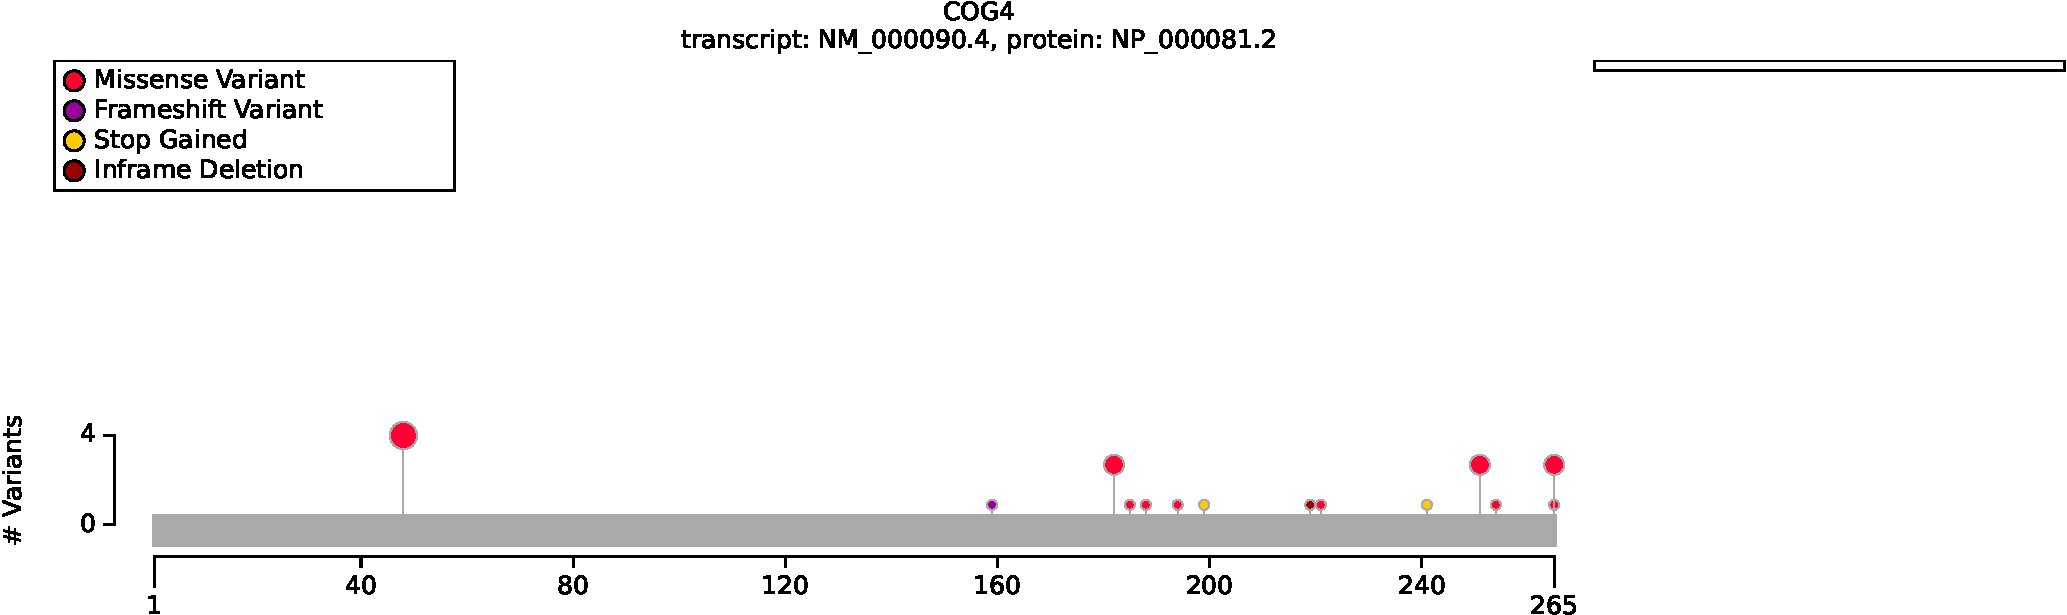
\includegraphics[width=\textwidth]{ img/COL3A1_protein_diagram.pdf} 
    \captionsetup{justification=raggedright,singlelinecheck=false}
    \caption{Distribution of variants in COL3A1}
    \end{subfigure}
    
    \vspace{2em}
    
    \begin{subfigure}[b]{0.95\textwidth}
    \centering
    \resizebox{\textwidth}{!}{
    \begin{tabular}{llllrr}
    \toprule
    Genotype (A) & Genotype (B) & total tests performed & significant results\\
    \midrule
    Missense & Other & 20 & 0\\
    Missense & Other & 20 & 0\\
    triple helix region & Other & 20 & 0\\
    OMIM:130050 & OMIM:618343 & 15 & 0\\
    Gly missense & Other & 20 & 0\\
    \bottomrule
    \end{tabular}
    }
    \captionsetup{justification=raggedright,singlelinecheck=false}
    \caption{ Fisher Exact Test performed to compare HPO annotation frequency with respect to genotypes. }
    \end{subfigure}
    
    \vspace{2em}
    
    \begin{subfigure}[b]{0.95\textwidth}
    \captionsetup{justification=raggedright,singlelinecheck=false}
    \resizebox{\textwidth}{!}{
    \begin{tabular}{llllrr}
    \toprule
    Description & Variable & Genotype (A) & Genotype (B) & p-value & xrefs\\
    \midrule
    Age of OMIM:130050 onset & Onset of OMIM:130050 & missense & other & 0.317 & -\\
    \bottomrule
    \end{tabular}
    }
    \caption{ Onset of OMIM:130050 to compare missense and other with respect to Onset of OMIM:130050. }
    \end{subfigure}
    
    \vspace{2em}
    
    \caption{ The cohort comprised 41 individuals (24 females, 17 males). A total of 43 HPO terms were used to annotate the cohort. Disease diagnoses: Ehlers-Danlos syndrome, vascular type (OMIM:130050) (35 individuals), Polymicrogyria with or without vascular-type EDS (OMIM:618343) (6 individuals). No significant GPC identified. Frank et al (2015) found that glycine missense variants were associated with a higher degree of severity in a cohort of 215 individuals. Primary data was not made available. A total of 38 unique variant alleles were found in \textit{COL3A1} (transcript: \texttt{NM\_000090.4}, protein id: \texttt{NP\_000081.2}).}
    \end{figure}
    